\chapter{Калибровка атомно-зондового томографа ПАЗЛ-3D}\label{ch:ch3}

\section{Верификация точности восстановления координат}\label{sec:ch3/sect1}

Определение пространственного разрешения атомно-зондового томографа обычно проводится при исследовании чистого металла с последующим анализом наличия/отсутствия атомных плоскостей. В случае, если пространственное разрешение установки равно или меньше чем расстояние между атомными плоскостями, разрешение установки считается равным или меньше чем расстояние атомными плоскостями, отвечающими тому или иному кристаллографическому направлению. Для верификации точности восстановления 3D координат был выбран поликристаллический вольфрам  \cite{scbibAPPLE}. Данный материал имеет ряд преимуществ для калибровочных процедур, таких как: отсутствие оксидного слоя, высокую температуру плавления, простоту изготовления образцов и кубическую объемно-центрированную решетку с параметром решетки 0.316 нм. Для подтверждения характеристик используется не менее 3 успешных исследований материала. Условия проведения исследования: температура образцов 22 К, частота работы лазера 25 кГц, мощность лазерного излучения не более 20 мВт, длина волны лазерного излучения 515 нм, скорость сбора данных от 60 до 250 событий/секунду. Пример полученного масс-спектра показан на рисунке \cref{fig:W_massspectr}. На масс-спектре отчетливо различимы пики всех стабильных изотопов вольфрама. Наблюдаемая зарядность ионов составила 3+. 

\begin{figure}[htb]
	\centerfloat{
		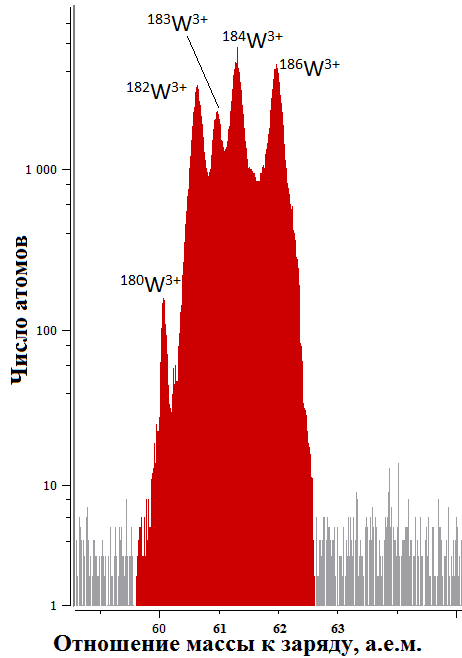
\includegraphics[width=.5\textwidth]{W_massspectr}
	}
	\caption{Масс-спектр образца из вольфрама}
	\label{fig:W_massspectr}
\end{figure}

Для оценки расстояния между атомными плоскостями были взяты отдельные части 3D объема в местах выхода кристаллографических направлений. Области выхода кристаллографических направлений определялись по двумерной гистограмме распределения событий на детектирующей системе, собранных за некоторый промежуток времени (Рисунок \cref{fig:W_3D}).

\begin{figure}[htb]
	\centerfloat{
		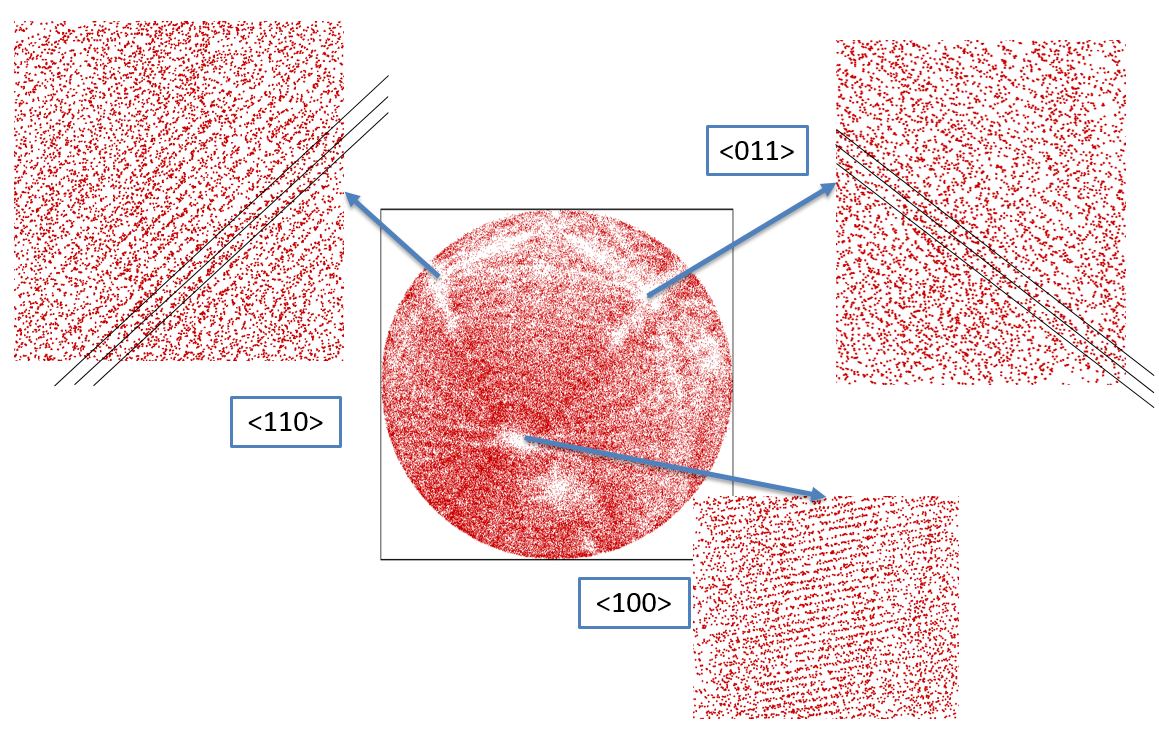
\includegraphics[width=\textwidth]{W_3D}
	}
	\caption{2D гистограмма распределения задетектированных событий}
	\label{fig:W_3D}
\end{figure}

Для каждого набора атомных плоскостей было определено среднее межплоскостное расстояние. Для выхода направления (100) измеренное расстояние составило 1.58 $\pm$ 0.03 \r{А}, что совпадает с табличным значение для вольфрама 1.58 \r{A} в переделах погрешности. Поскольку в данных исследованиях выход (100) ориентирован вдоль оси образца, то способность установки наблюдать атомные плоскости позволяет оценить разрешающую способность прибора вдоль оси образца (Z) в не более чем 1-2 \r{A}. Для выходов (011) также было измерено межплоскостное расстояние: 1.9 $\pm$ 0.3 \r{A}, что также согласуется с табличным значением в 2.23 \r{A}. Наборы плоскостей (011) и (110) расположены под углом к оси образца, это позволяет оценить латеральное разрешение установки: 2-4 \r{A}. Полученные оценки разрешающей способности ПАЗЛ-3D  характерны для большинства атомно-зондовых томографов. 

\FloatBarrier

\section{Определение оптимальной метрики качества испарения}\label{sec:ch3/sect3}

В ходе сбора данных с одного образца ряд факторов может приводить к изменению условий испарения атомов материала. Например, происходит изменение формы кончика образца (так как он постепенно испаряется), может происходить медленный <<дрейф>>  мощности лазера или фокусировка лазерного излучения может выйти из оптимального положения. Данные изменения приводят к различным отклонениям в испарении, которые будут влиять на результат анализа данных. Следовательно, для проведения количественных исследований необходимо разработать методику поддержания постоянных и воспроизводимых условий испарения в рамках исследования одного образца. В разделе \cref{sec:ch1/sec5} описаны основные используемые метрики для сравнения АЗТ данных. Поскольку ПАЗЛ-3D это новая разработанная установка, то необходимо разработать методику сравнения результатов исследований для обеспечения воспроизводимости получаемых данных.

Для отработки данной методики был выбран сплав Al-3.5Cu-0.2Mn-0.1S~wt\%. Это однородный материал на масштабах нескольких сотен нанометров. Также стоит отметить, что это 4-компонентный сплав, что дает возможность проследить изменения концентраций нескольких элементов друг относительно друга при различных условиях испарения. Исследования проводились при постоянной температуре образца 50 К. Остальные параметры менялись в ходе сбора данных. В начале работы были выбраны несколько различных метрик-кандидатов для оценки пригодности для контроля условий испарения. Ниже приведен список возможных метрик:

\begin{itemize}
	\item Концентрации элементов,
	\item Мощность лазерного излучения,
	\item Доля однократных событий (или общая доля мультисобытий),
	\item Доля мультисобытий одного из элементов,
	\item Соотношение зарядностей основного элемента,
	\item Доля шум до пика основного элемента (10-11 а.е.м.),
	\item Доля шум после пика основного элемента (40-41 а.е.м.).		
\end{itemize}

К метрикам предъявлялось несколько требований. Первое и основное - корректность получаемых концентраций элементов. Второе, не менее важное требование, это возможность вычислять значение выбранной метрики <<in-situ>> в процессе сбора данных. Также требовалась минимальная повторяемость результатов, хотя бы в рамках одного исследования. Для оценки повторяемости значений метрик данные собирались в определенном порядке. Основным варьируемым параметром являлась мощность лазерного излучения. Соответственно, в ходе исследований мощность сначала поэтапно уменьшали, потом увеличивали, затем опять уменьшали. Это позволило оценить возможность воспроизводить условия испарения на протяжении всего сбора данных. В таблицах Приложения \cref{app:B} приведены все параметры проведения исследований и результаты расчета значений выбранных метрик. Далее в работе показаны основные зависимости, которые были обнаружены или наличие которых было подтверждено (ранее они описывались для других атомно-зондовых томографов).

Наиболее очевидной и ожидаемой являлась зависимость детектируемой концентрации от мощности лазерного излучения. Точки зависимости приведены на Рисунках  \cref{fig:params_Conc_Power}, где точки соединены в порядке сбора данных.  Зависимость концентрации элемента практически прямо пропорциональна мощности лазерного излучения. Но в случае другой фокусировки лазера, а следовательно и другой мощности излучения лазера, уже наблюдается нелинейная зависимость (рисунок \cref{fig:params_Conc_Power} б)). Скорее всего есть область оптимума точности сбора данных между слишком малой и слишком большой мощностями лазерного излучения. Данное предположение коррелирует с наблюдаемыми зависимостями качества данных в работе \cite{scbibOptParamsYAFI} (подробно описывалось в разделе \cref{sec:ch1/sec5}).

\begin{figure}[htb]
	\begin{minipage}[b]{0.49\textwidth}\centering
		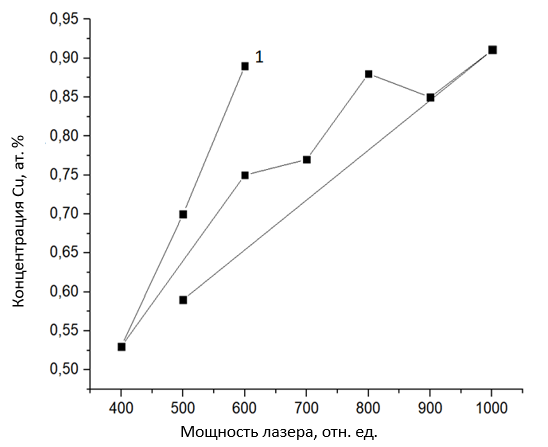
\includegraphics[width=\textwidth]{params_Conc_Power} \\ а)
	\end{minipage}
	\begin{minipage}[b]{0.49\textwidth}\centering
		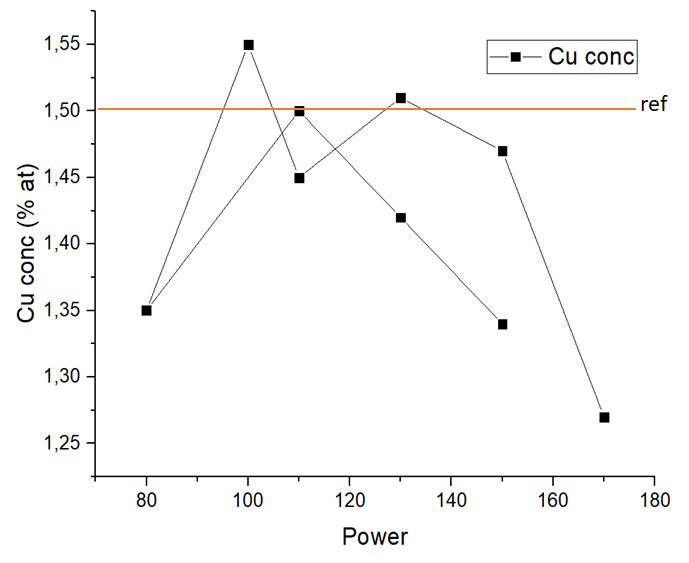
\includegraphics[width=\textwidth]{params_Conc_Power_2} \\ б)
	\end{minipage}
	\caption{Значения концентрации Cu при различной мощности лазерного излучения для двух наборов исследований. Точки соединены в порядке сбора данных. Оранжевой горизонтальной линией на отмечено табличное значение концентрации меди для исследуемого материала}
	\label{fig:params_Conc_Power}
\end{figure}

\FloatBarrier

Важно отметить, что данные для Рисунка \cref{fig:params_Conc_Power} были обработаны уже после проведения исследований. Как выше было неоднократно отмечено, что напрямую концентрации в процессе сбора данных затруднительно вычислять точно, с учетом шума/коррекций/оптимизаций.

Далее изучим другую, более перспективную метрику, основанную на соотношении зарядностей. Поскольку основным элементом в данном материале является алюминий, то была оценена зависимость концентрации меди от отношения $Al^{+}/Al^{++}$ (Рисунок \cref{fig:params_Conc_CSR}).

\begin{figure}[htb]
	\begin{minipage}[b]{0.49\textwidth}\centering
		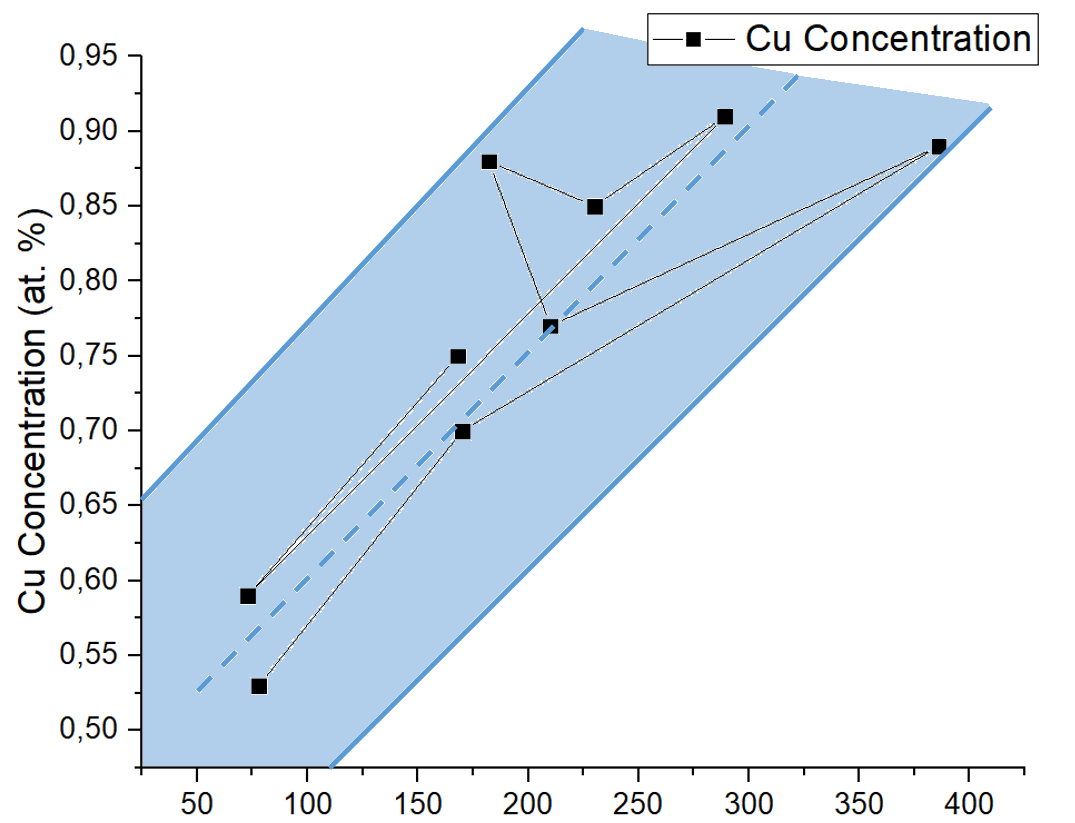
\includegraphics[width=\textwidth]{CSR_1} \\ а)
	\end{minipage}
	\begin{minipage}[b]{0.49\textwidth}\centering
		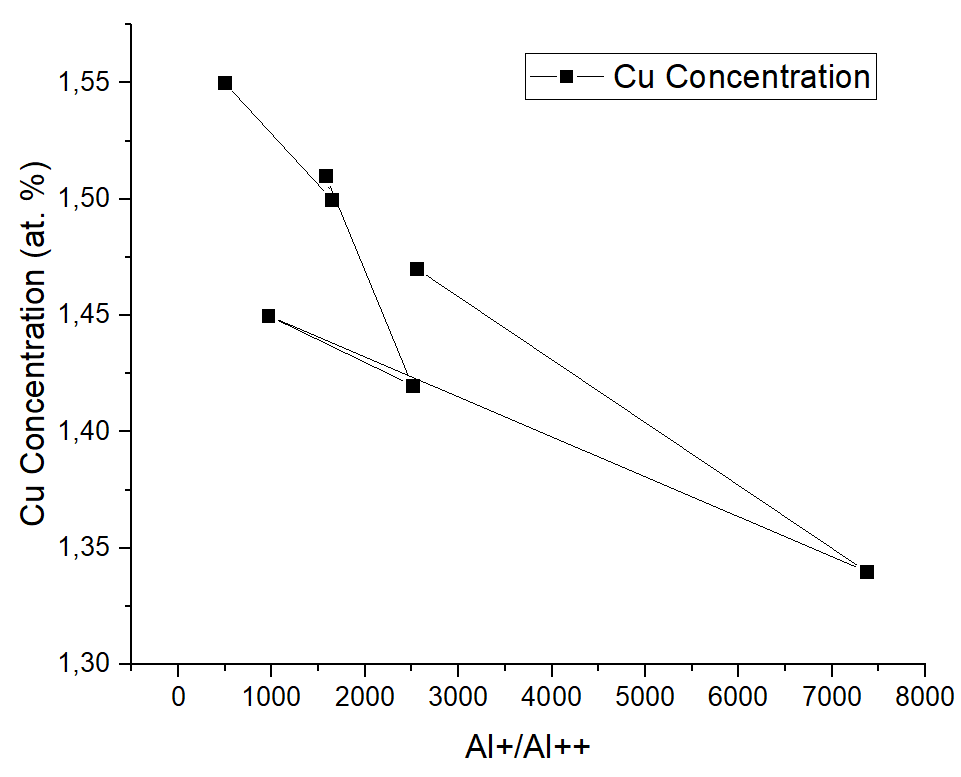
\includegraphics[width=\textwidth]{CSR_2} \\ б)
	\end{minipage}
	\caption{Значения концентрации Cu при различном соотношении зарядностей алюминия для двух наборов исследований. Точки соединены в порядке сбора данных.}
	\label{fig:params_Conc_CSR}
\end{figure}

На Рисунке \cref{fig:params_Conc_CSR} наглядно видно, что для первого набора данных в области значений $Al^{+}/Al^{++}$ от 75 до 400 концентрация меди не достигает требуемого значения в 1.52 ат. \%, но при этом явно наблюдается воспроизводимость значения концентрации при похожих значениях соотношения зарядностей. Наблюдаемую зависимость можно аппроксимировать линейной функцией ($y = ax + b$) с параметрами a = XXX, b = YYYYY. При этом для второго набора данных наблюдается противоположный характер зависимости. В этом случае можно также провести аппроксимацию линейной зависимостью с параметрами a = XXX, b = YYYYY. Стоит отметить, что во втором наборе данных 2 промежуточные точки практически с идеальной точностью соответствуют табличному значению концентрации меди в данном материале. Аналогичный характер зависимостей наблюдался в работе \cite{Mancini14}, что подтверждает корректность предложенной методики. Для второго набора данных также построены значения концентраций других элементов  в зависимости от соотношения зарядностей алюминия ( Рисунок \cref{fig:params_Sn_Mn_O}).

\begin{figure*}
	\centering
	\begin{subfigure}[b]{0.475\textwidth}
		\centering
		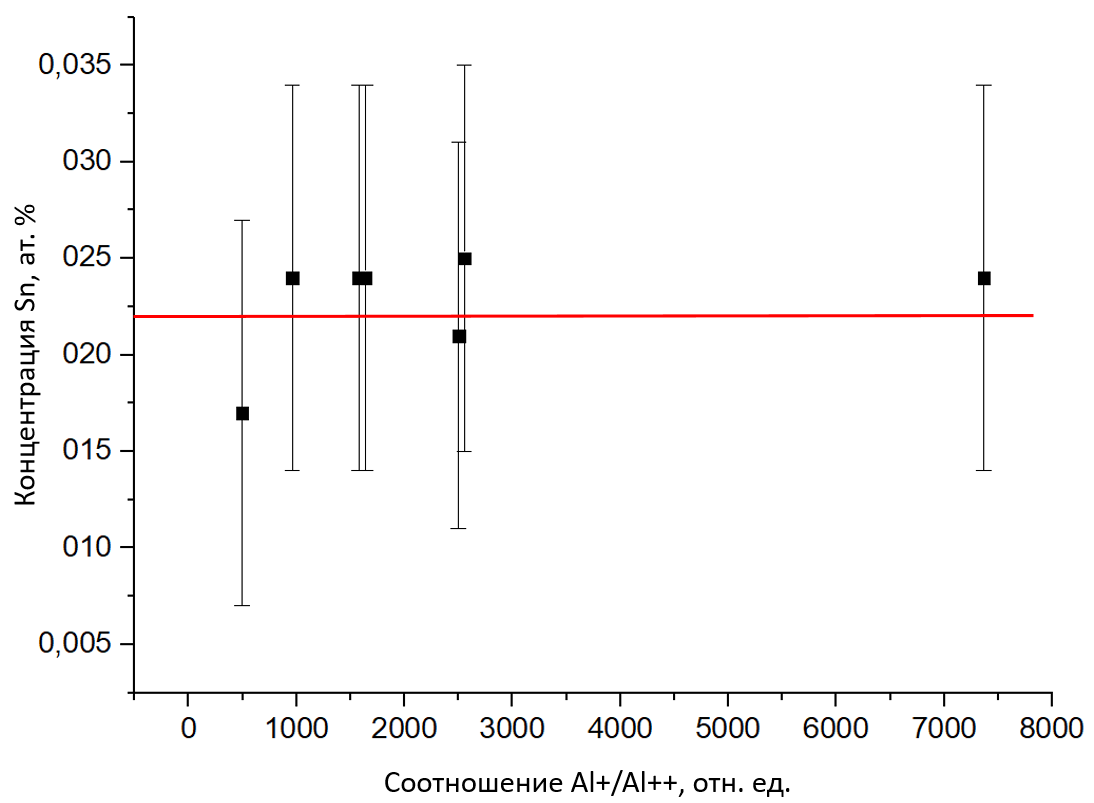
\includegraphics[width=\textwidth]{params_sn_conc}
		\caption{}    
	\end{subfigure}
	\hfill
	\begin{subfigure}[b]{0.475\textwidth}  
		\centering 
		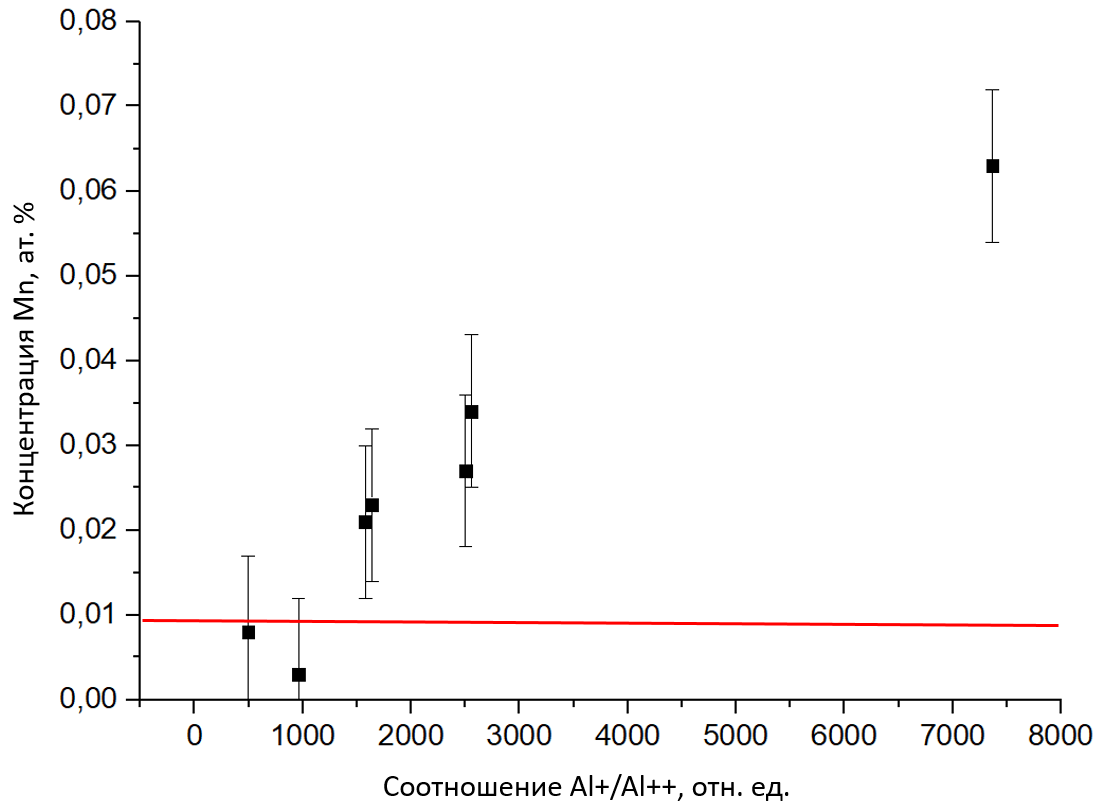
\includegraphics[width=\textwidth]{params_mn_conc}
		\caption{}    
	\end{subfigure}
	\vskip\baselineskip
	\begin{subfigure}[b]{0.475\textwidth}   
		\centering 
		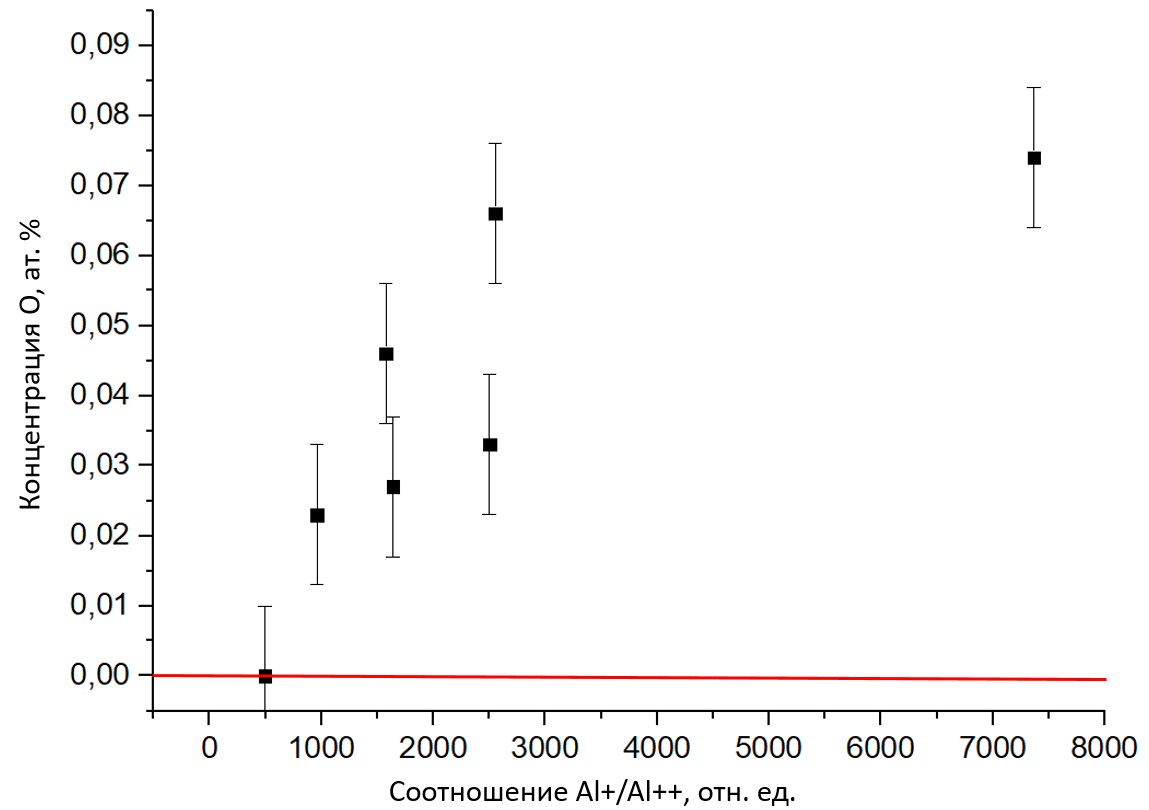
\includegraphics[width=\textwidth]{params_o_conc}
		\caption{}    
	\end{subfigure}
	\hfill
	\caption
	{Значения концентраций Sn (а), Mn (б), O (в) в зависимости от соотношения зарядностей алюминия. Красной линией указаны ожидаемые значения концентрации для исследуемого материала   } 
	\label{fig:params_Sn_Mn_O}
\end{figure*}

Анализируя результаты, показанные на Рисунках \cref{fig:params_Conc_CSR,fig:params_Sn_Mn_O} можно заключить, что для установки ПАЗЛ-3D для алюминиевого сплава Al-3.5Cu-0.2Mn-0.1S~wt\% оптимальным диапазоном значений соотношения зарядностей является промежуток от 300 до 2000 отн. еди. В данном промежутке концентрации меди и олова наиболее близки к табличным значениям. При этом наблюдается малое количество кислорода, наличие которого является артефактом лазерного испарения. Таким образом показано, что соотношение зарядностей основного элемента может служить метрикой качества данных. Показана воспроизводимость результатов исследований с использованием контроля условий испарения по соотношению зарядностей основного элемента.

При оценке зависимости качества АЗТ данных от других метрик было продемонстрировано несколько второстепенных зависимостей (или показано их отсутствие) для сплава Al-3.5Cu-0.2Mn-0.1S~wt\%:

\begin{itemize}
	\item Доля мультисобытий не является воспроизводимой метрикой для АЗТ данных,
	\item Мощность лазерного излучения пропорциональная соотношению зарядностей, но имеет плохую воспроизводимость на разных наборах данных, а следовательно точно не подходит для разных установок (Рисунок \cref{fig:params_Noise_Multi} в)),	
	\item Доля мультисобытий меди имеет тенденцию к снижению с ростом напряжения на образце,
	\item Доля шум до пика основного элемента (10-11 а.е.м.) и доля шум после пика основного элемента (40-41 а.е.м.)	падают с увеличением мощности лазерного излучения и увеличиваются с ростом напряжения на образце (Рисунок \cref{fig:params_Noise_Multi} а) и б)),
	\item Доля мультисобытий меди не является воспроизводимой метрикой для АЗТ данных.	
\end{itemize}

Полученные второстепенные зависимости могут быть важны для более оптимального выбора условий испарения в дальнейших работах по развитию методик исследования алюминиевых сплавов. Также полученные корреляции могут использоваться для лучшей интерпретации данных. Все указанные метрики собраны в Таблице \cref{tab:params_expl}, в которой также приведены основные их особенности как кандидатов для основной метрики качества и воспроизводимости данных.

\begin{figure*}
	\centering
	\begin{subfigure}[b]{0.475\textwidth}
		\centering
		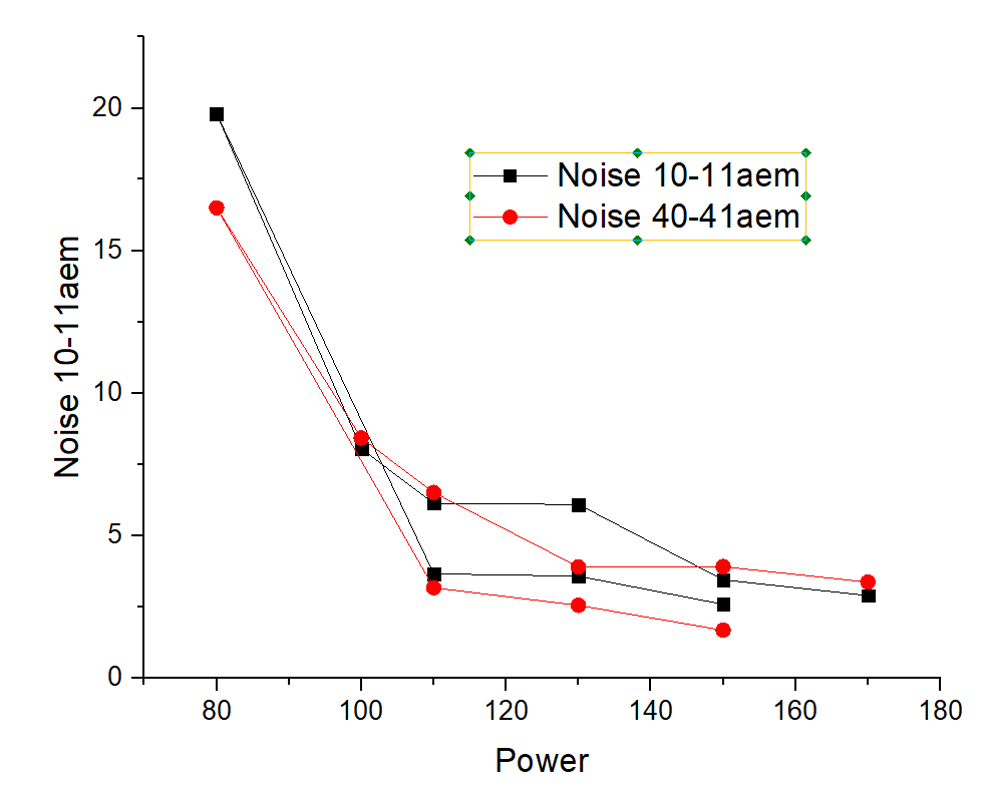
\includegraphics[width=\textwidth]{params_Noise_Power}
		\caption{}    
	\end{subfigure}
	\hfill
	\begin{subfigure}[b]{0.475\textwidth}  
		\centering 
		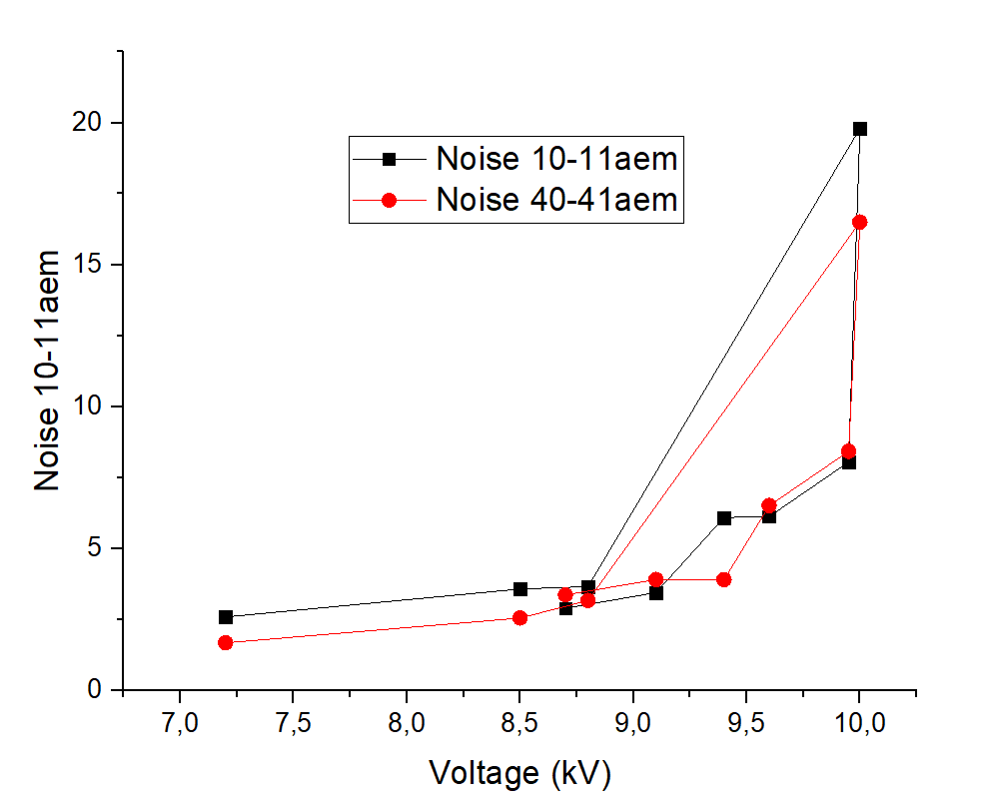
\includegraphics[width=\textwidth]{params_Noise_Voltage}
		\caption{}    
	\end{subfigure}
	\vskip\baselineskip
	\begin{subfigure}[b]{0.475\textwidth}   
		\centering 
		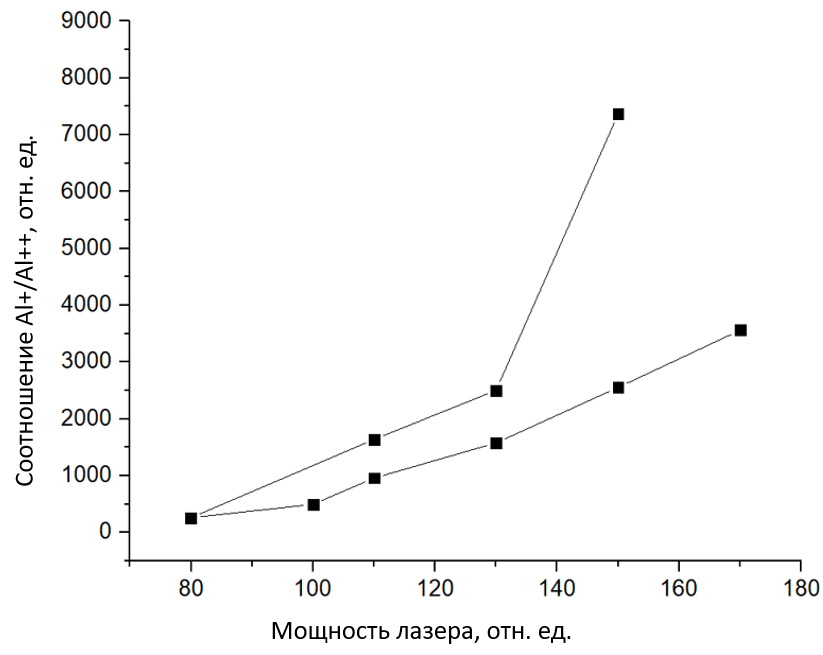
\includegraphics[width=\textwidth]{params_CSR_Power}
		\caption{}    
	\end{subfigure}
	\hfill
	\caption
	{а) - Значения шума до и после пика основного элемента от мощности лазерного излучения. б) - - Значения шума до и после пика основного элемента от напряжения на образце. в) Значения соотношения зарядностей в зависимости от мощности лазерного излучения. На всех рисунках точки соединены в порядке сбора данных} 
	\label{fig:params_Noise_Multi}
\end{figure*}

\begin{table} [htb]
	\centering
	\caption{Метрики качества атомно-зондовых данных}
	\label{tab:params_expl}
	\begin{SingleSpace}
		\begin{tabularx}{\textwidth} {| X | X | X | X |}
			\hline
			Наименование & Описание/ комментарии & Возможная интерпретация & Минусы  \\ \hline
			Однократные события & {Доля однократных событий ко всем событиям}  & {Чем больше - тем проще расшифровывать данные}  & {Нет прямой корреляции с концентрациями}              \\ \hline
			Мощность лазера & {Легко измеряется/ меняется в процессе исследования}  & {-}  & {нет повторяемости от образца к образцу}              \\ \hline
			Доля мультисобытий Cu & Возможная метрика сложности точности определения концентрации & Чем меньше - тем лучше & Нет прямой корреляции с концентрациями          \\ \hline		
			Шум до пиков основного элемента сплава      & Доля атомов с массами от 10 до 11 а.е.м. & Чем больше мощность лазера, тем меньше шума, чем выше напряжение, тем больше шума  & Нет прямой корреляции с концентрациями               \\ \hline
			Шум после пиков основного элемента сплава     & Доля атомов с массами от 40 до 41 а.е.м. & Чем больше мощность лазера, тем меньше шума, чем выше напряжение, тем больше шума  & Нет прямой корреляции с концентрациями             \\ \hline
			Концентрации  & -   &  -   & Расчет невозможен в реальном времени  \\ \hline			
			Соотношение зарядностей основного элемента Al$^+$/Al$^{++}$, отн. ед.    & Возможна оценка по предварительному масс-спектру, без оптимизации   & Есть значимая зависимость и повторяемость концентраций от соотношения зарядностей  & Может отличаться для разных материалов   \\ \hline
		\end{tabularx}
	\end{SingleSpace}
\end{table}

\FloatBarrier
Таким образом, в данном разделе продемонстрирована методика выбора метрики качества и воспроизводимости АЗТ данных для алюминиевых сплавов. Показано, что предпочтительная метрика, основанная на соотношение зарядностей для основного химического элемента материала. Основываясь на том, что сохранение соотношения зарядностей основного химического элемента обеспечивают воспроизводимость результатов АЗТ исследований (концентрации близки к ожидаемым), можно заключить, что методика поиска оптимальных параметров испарения включает следующее:

\begin{itemize}
	\item сбор набора АЗТ данных при различных соотношения зарядностей основного химического элемента,
	\item расчет концентрации всех элементов,	
	\item (дополнительно) проверка данных на отсутствие артефактов испарения (например, наличия кислорода, не входящего в состав материала),
	\item в случае неполучения целевых значений концентраций или наличия большого числа артефактов проверка более широкого диапазона значений соотношений зарядностей,
	\item выбор диапазона значений соотношений зарадностей, при котором концентрации наиболее близки к целевым значениям и при этом наблюдается минимальное количество артефактов испарения.	
\end{itemize}
В дальнейших исследованиях сплавов данного типа можно придерживаться выбранного диапазона значений соотношений зарядностей.

\FloatBarrier

\section{Сравнение атомно-зондовых данных, полученных на установках ПАЗЛ-3D и АТЛАЗ на примере сплава Al-Cu-Zr}\label{sec:ch3/sect4}

Для демонстрации методики сравнения АЗТ данных, описанной в предыдущем разделе \cref{sec:ch3/sect3} было проведены исследования на двух АЗТ установках с лазерным испарением ПАЗЛ-3D и АТЛАЗ (Модернизированная АЗТ установка АТЛАЗ была собрана на базе прибора CAMECA ECOTAP). Для исследования выбирались материалы содержащие различные наноразмерные кластеры. Одним из материалов была выбрана сталь 16Х12МВСФБР ЭП-823 \cite{Porollo04} после облучения ионами (далее ЭП-823). Данная сталь отличается высокой плотность кластеров. Вторым материалом для сравнения выбран алюминиевый сплав Al-3.3Cu-2.5Mn-0.5Zr (мас. \%) после отжига при температурах 350 \textdegree С и 450 \textdegree С \cite{Belov22,Belov21} (далее сокращенно называются как Al-Cu-Mn-Zr 350 \textdegree С и Al-Cu-Mn-Zr 450 \textdegree С, соответственно). Основной задачей данного сравнения было демонстрация работоспособности методики, описанной в предыдущем разделе, для других материалов. Стоит отметить, что данная проверка проводилась для материалов без больших (более 1 мкм) структурных объектов. 

Поскольку данные исследования проводились на стадии отработки методики, то контролировалось больше технических параметров исследования, чем это было бы необходимо для обычных исследований <<на поток>>. В качестве метрик сравнения исследований использовались как общепринятые параметры, так и ряд технических характеристик данных, которые в обычных исследованиях используются редко. Обычно при анализе АЗТ данных в результатах приводятся концентрации химических элементов в матрице материала, в концентрации в кластерах, размеры кластеров и их объемная плотность. В данных исследованиях к этим метрикам был добавлен ряд таких параметров как: соотношение зарядностей основного элемента, разрешение по массе на полувысоте пика, разрешение по массе на 10~\% высоты пика, общий процент мульти-событий, доля мульти-событий, приходящаяся на элементы, которые являются кластеро-/фазо-образующими, скорость детектирования и уровень шума.  В таблицах \cref{tab:paramsAPPLEvsATLAS,tab:matrixAPPLEvsATLAS,tab:clustersAPPLEvsATLAS}, представлено сравнение значений метрик на разных установках для алюминиевого сплава.

\begin{table} [htbp]
	\centering
	\caption{Сравнение характеристик точности восстановления данных для алюминиевых сплавов Al-Cu-Mn-Zr}
	\label{tab:paramsAPPLEvsATLAS}
	\begin{SingleSpace}
		\begin{tabular} {| c | c | c | c | c |}
			\hline
			{} & \thead{ПАЗЛ-3D, \\350 \textdegree C} & \thead{АТЛАЗ, \\350 \textdegree C} & \thead{ПАЗЛ-3D, \\450 \textdegree C} & \thead{АТЛАЗ, \\450 \textdegree C} \\ \hline
			$M/\Delta M_{50\%}$ Al$^+$ & 670  & 260  & 421  & 430               \\ \hline
			$M/\Delta M_{10\%}$ Al$^+$ & 206  & 120  & 146  & 190               \\ \hline
			Мульти-события, \%         & 0.7  & 2.9  & 0.9  & 2.9               \\ \hline
			Мульти-события Cu, \%      & 4.23 & 0.54 & 7.11 & 3.17              \\ \hline
			Мульти-события Zr, \%      & 7.31 & 0.85 & 0.18 & 0.6               \\ \hline
			Шум, 10$^{-5}$ отн. ед. & 5.4   & 1.9   & 10.7  & 1.67  \\ \hline
			Скорость сбора данных, атомов/возд.        & 0.005 & 0.006 & 0.007 & 0.007 \\ \hline
			Соотношение Al$^+$/Al$^{++}$, отн. ед.    & 640   & 310   & 630   & 450   \\ \hline
		\end{tabular}
	\end{SingleSpace}
\end{table}

Образцы для АЗТ исследования были изготовлены с помощью электроэрозионной резки, с последующим электрохимическим утонением. В процессе сбора данных температура образцов поддерживалась равной 50~К. Мощность лазера на  ПАЗЛ-3D составляла 85 $\pm$ 1 мВт, а на АТЛАЗ - 3.0 $\pm$ 0.5 мВт. Скорость сбора данных представлена в Таблице \cref{tab:paramsAPPLEvsATLAS}. Обработка и восстановление АЗТ данных проводилась с помощью ПО <<КВАНТМ-3D>>. Параметры 3D восстановления были выбраны с помощью методики, описанной в работе \cite{scbibDensity}. Полевой фактор $k_f$ для всех исследований находится в диапазоне от 4 до 6, коэффициент сжатия изображения ICF  - от 1.2 до 1.6. Масс-спектр восстанавливался по методике, представленной в работе \cite{Shutov19}. Атомные карты представлены на Рисунке.  \cref{fig:APPLEvsATLAS}.



Концентрации и их погрешности был для всех исследований были рассчитаны по формулам, предложенным в работах Danoix \cite{Danoix071,Danoix072}. В случае, если на одно состояние приходилось более одного исследования, то в качестве погрешности указано среднее отклонение от среднего значения. 





Для Al-Cu-Mn-Zr 450~\textdegree C на ПАЗЛ-3D представлены средние значения характеристик данных по трем исследованным образцам. Проведено сравнение химического состава материалов как в кластерах для Al-Cu-Mn-Zr 350~\textdegree C, так и в матрице для Al-Cu-Mn-Zr 350~\textdegree C и 450~\textdegree C. Ввиду не сферичной формы включений Zr была использована методика изо-концентрационных поверхностей (поверхностей одинаковой концентрации). Для определений границ включений были построены поверхности так, чтобы перегиб профиля концентраций, построенный нормально к поверхности (проксиграмма) проходил точно на полувысоте по концентрациям \cite{Hellman07}. Параметры, используемые для построения и расчетов, были выбраны следующие: размер сетки 1-1.5 нм, делокализация 2 нм, изо-концентрация поверхности по 1.5 \% Zr. 

\begin{table} [htbp]
	\centering
	\caption{Состав кластеров [ат. \%] в алюминиевом сплаве Al-Cu-Mn-Zr после отжига при 350~\textdegree C, полученный
		на установках ПАЗЛ-3D и АТЛАЗ}
	\label{tab:clustersAPPLEvsATLAS}
	\begin{SingleSpace}
		\begin{tabular} {| c | c | c |}
			\hline
			{} & ПАЗЛ-3D & АТЛАЗ \\ \hline
			Al       & 96.9 $\pm$ 0.3  & 99.7 $\pm$ 0.4   \\ \hline
			Cu       & 0.3 $\pm$ 0.1   & 0.3 $\pm$ 0.1    \\ \hline
			Mn       & 0.04 $\pm$ 0.02 & 0.003 $\pm$ 0.002  \\ \hline
			Zr       & 2.4 $\pm$ 0.3   & 2.8 $\pm$ 0.2    \\ \hline
			Ni, C, O & Баланс & Баланс   \\ \hline			
		\end{tabular}
	\end{SingleSpace}
\end{table}

\begin{table} [htbp]
	\centering
	\caption{Состав матрицы [ат. \%] в алюминиевых сплавах Al-Cu-Mn-Zr после отжига при 350~\textdegree C и при 450~\textdegree C, полученный
		на установках ПАЗЛ-3D и АТЛАЗ}
	\label{tab:matrixAPPLEvsATLAS}
	\begin{SingleSpace}
		\begin{tabular} {| c | c | c | c | c |}
			\hline
			{} & \thead{ПАЗЛ-3D, \\ 350~\textdegree C} & \thead{АТЛАЗ, \\ 350~\textdegree C} & \thead{ПАЗЛ-3D, \\ 450~\textdegree C} & \thead{АТЛАЗ, \\ 450~\textdegree C} \\ \hline
			Al       & 99.49 $\pm$ 0.01  & 99.66 $\pm$ 0.01 & 99.2 $\pm$ 0.1  & 99.20 $\pm$ 0.01  \\ \hline
			Cu       & 0.29 $\pm$ 0.06   & 0.24 $\pm$ 0.04  & 0.6 $\pm$ 0.2  & 0.67 $\pm$ 0.05  \\ \hline
			Mn       & 0.01 $\pm$ 0.01 & 0.004 $\pm$ 0.002 & 0.02 $\pm$ 0.01  & 0.010 $\pm$ 0.005 \\ \hline
			Zr       & 0.11 $\pm$ 0.05   & 0.06 $\pm$ 0.04 & 0.010 $\pm$ 0.008  & 
			0.08 $\pm$ 0.05   \\ \hline
			Ni, C, O & Баланс & Баланс & Баланс & Баланс  \\ \hline			
		\end{tabular}
	\end{SingleSpace}
\end{table}


\begin{figure}[h!tb]
	\begin{minipage}[b][][b]{0.49\textwidth}\centering
		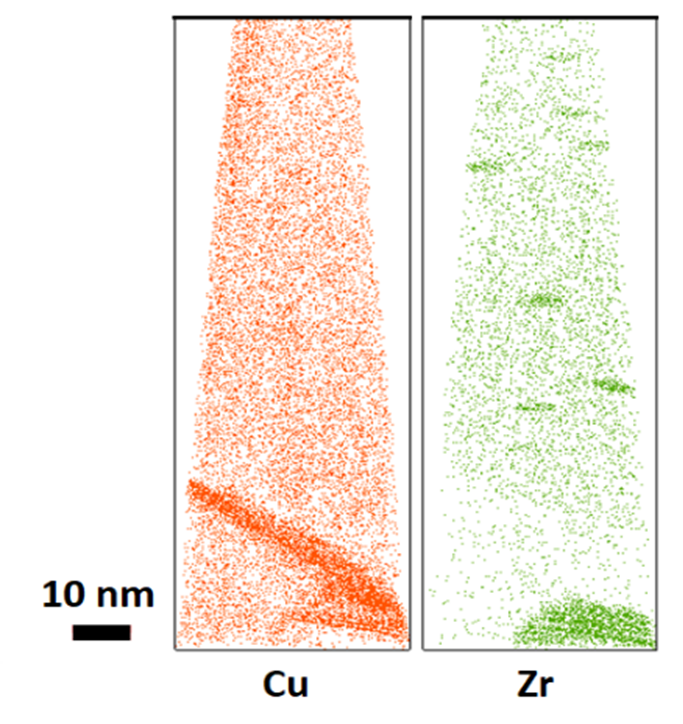
\includegraphics[scale=0.5]{APPLEvsATLAS_apple} \\ а)
	\end{minipage}
	%\hfill
	\begin{minipage}[b][][b]{0.49\textwidth}\centering
		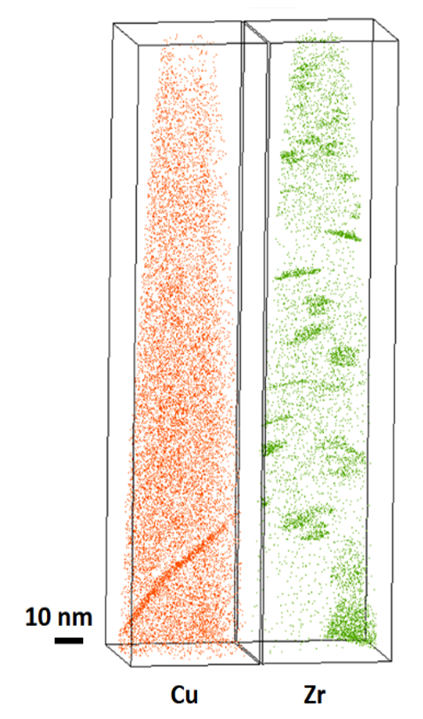
\includegraphics[scale=0.8]{APPLEvsATLAS_atlas} \\ б)
	\end{minipage}
	\caption{а) Атомные карты сплава Al-Cu-Mn-Zr 350~\textdegree C ПАЗЛ-3D. б) Атомные карты сплава Al-Cu-Mn-Zr 350~\textdegree C АТЛАЗ.}
	\label{fig:APPLEvsATLAS}
\end{figure} 

Данные для Al-Cu-Mn-Zr 450~\textdegree C на ПАЗЛ-3D рассчитаны как среднее по трем исследованным образцам, погрешности также для данного материла рассчитаны как среднее отклонение от среднего значения. Плотность включений для данных с ПАЗЛ-3D составила (0.9 $\pm$ 0.1) x 10$^{23}$ и (1.40 $\pm$ 0.05) x 10$^{23}$ штук в м$^3$ для АТЛАЗ.

Исследование ЭП-823
Условия сбора данных были во много идентичны тем, что использовались при исследовании алюминиевых сплавов. Температура образцов составляла 50~К, мощность лазера на ПАЗЛ-3D 40 $\pm$ 1 мВт, на АТЛАЗ 2 $\pm$ 0.5 мВт. Для восстановления атомно-зондовых данных и их обработки также использовалось ПО КВАНТМ~3D и те же алгоритмы 3D восстановления. Множитель поля $k_f$ составлял 4.5, коэффициент сжатия изображения ICF от 1.2 до 1.35. Процесс обработки масс-спектра включал в себя первоначальную разметку с помощью автоматизированного инструмента разметки модуля “environment editor”, после была проведена ручная коррекция размеченных пиков. Далее был проведен пересчет пресекающихся пиков, в частности для Cr и Fe, ориентируясь на соседние пики этих элементов. Был проведен пересчет коэффициента Ni++ с целью минимизировать влияние термического хвоста Fe. Пики меди были разделены и рассмотрены на 3D модели, с целью убедиться, что оба пика соответствуют Cu. Также были проверены пики Mo на возможное пересечение с Cr+. В образце на ПАЗЛ-3D, был обнаружен пик Nb между пиками Mo, на АТЛАЗ из-за повышенного шума этот пик не виден на масс-спектре. На Рисунке \cref{fig:APPLEvsATLAS_EP} показаны атомные карты объемов.

\begin{figure}[h!tb]
	\begin{minipage}[b][][b]{0.49\textwidth}\centering
		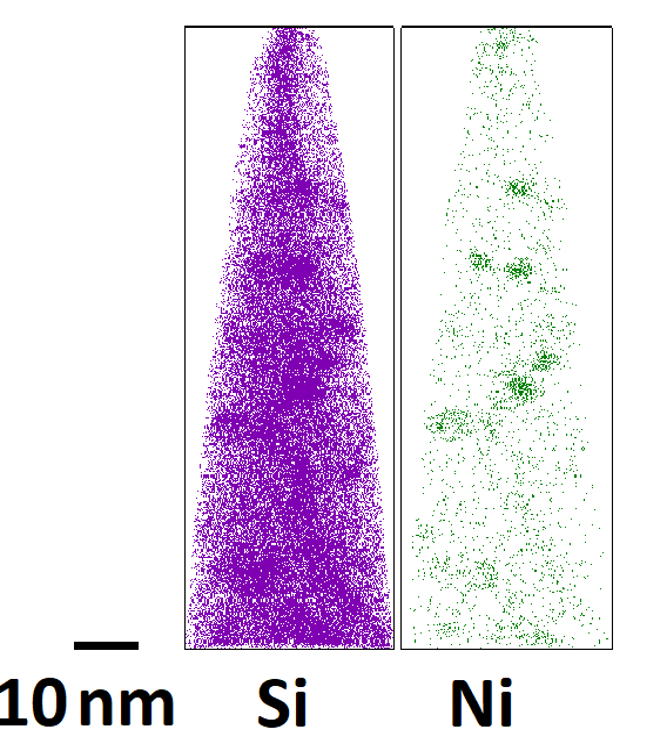
\includegraphics[scale=0.5]{APPLEvsATLAS_apple_EP} \\ а)
	\end{minipage}
	%\hfill
	\begin{minipage}[b][][b]{0.49\textwidth}\centering
		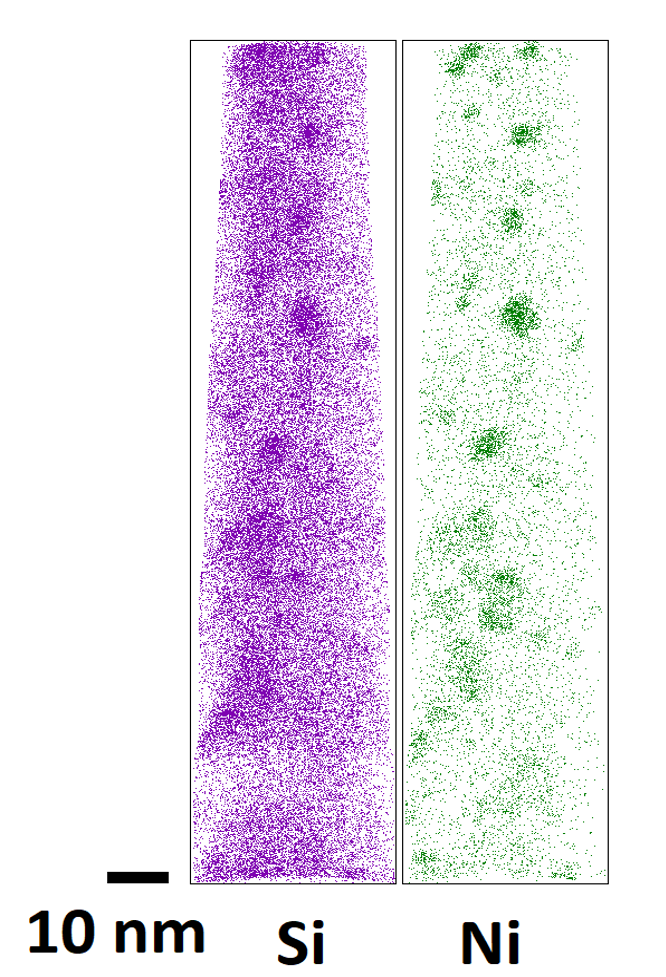
\includegraphics[scale=0.8]{APPLEvsATLAS_atlas_EP} \\ б)
	\end{minipage}
	\caption{Атомные карты облученной стали ЭП-823 на ПАЗЛ-3D (а) и АТЛАЗ (б).}
	\label{fig:APPLEvsATLAS_EP}
\end{figure} 

Поиск кластеров был проведен по Ni+ согласно алгоритму максимального разделения [ссылка на максимальное разделение]. Из пересечения соответствующих графиков, получены параметры идентификации кластеров по методу максимальной сепарации ($N_min$ = 7 и R = 8 для ПАЗЛ-3D и $N_min$ = 7 и R = 7.5 для АТЛАЗ). По найденным параметрам были выделены кластеры, после их отделения от матрицы. Были просмотрены кластеры на 3D изображении для выявления случайного объединения или выделения несоответствующий области в качестве кластера. Был создан отдельный масс-спектр для кластеров. В этом масс-спектре учитывались в приоритете элементы обогащения, в частности Ni++. Также внутри кластеров для обеих установок был обнаружен Nb и, соответственно, размечен. Данные масс-спектра отдельно матрицы и кластеров были экспортированы и объединены в общей таблице. В Таблицах \cref{tab:paramsAPPLEvsATLAS_EP3,tab:matrix_clustersAPPLEvsATLAS}, представлено сравнение данных для разных установок отдельно для стали ЭП-823.

\begin{table} [htbp]
	\centering
	\caption{Сравнения характеристик точности восстановления данных для ЭП-823 на установках ПАЗЛ-3D и АТЛАЗ}
	\label{tab:paramsAPPLEvsATLAS_EP3}
	\begin{SingleSpace}
		\begin{tabular} {| c | c | c |}
			\hline
			{}                                     & ПАЗЛ-3D & АТЛАЗ   \\ \hline
			$M/\Delta M_{50\%}$ Al$^+$             & 938     & 726     \\ \hline
			$M/\Delta M_{10\%}$ Al$^+$             & 245     & 329     \\ \hline
			Мульти-события, \%                     & 1.4     & 17.7                 \\ \hline
			Мульти-события Ni, \%                  & 1.7     & 28.6             \\ \hline
			Мульти-события Si, \%                  & 0.4     & 26.1             \\ \hline
			Мульти-события Cu, \%                  & 3.9     & 6.7             \\ \hline
			Шум, 10$^{-5}$ отн. ед.                & 10.05   & 30.1     \\ \hline
			Скорость сбора данных, атомов/возд.    & 0.008   & 0.01  \\ \hline
			Соотношение Al$^+$/Al$^{++}$, отн. ед. & 307     & 368     \\ \hline
		\end{tabular}
	\end{SingleSpace}
\end{table}

\begin{table} [htbp]
	\centering
	\caption{Сравнение состава матрицы [ат. \%] для алюминиевых сплавов Al-Cu-Mn-Zr после отжига при температурах 350 °С и 450 °С, полученных на установках ПАЗЛ-3D и АТЛАЗ}
	\label{tab:matrix_clustersAPPLEvsATLAS}
	\begin{SingleSpace}
		\begin{tabular} {| c | c | c | c | c |}
			\hline
			{} & \thead{ПАЗЛ-3D матрица} & \thead{АТЛАЗ матрица} & \thead{ПАЗЛ-3D кластеры} & \thead{АТЛАЗ кластеры} \\ \hline
			Fe       & 83.43 $\pm$ 0.02 & 83.98 $\pm$ 0.02  & 48 $\pm$ 1      & 53 $\pm$ 1  \\ \hline
			Cr       & 11.11 $\pm$ 0.06 & 10.51 $\pm$ 0.05  & 6.9 $\pm$ 0.8   & 7.3 $\pm$ 0.7   \\ \hline
			Si       & 2.59 $\pm$ 0.06  & 1.88 $\pm$ 0.05   & 15 $\pm$ 1      & 10.0 $\pm$ 0.8 \\ \hline
			Mn       & 0.94 $\pm$ 0.06  & 1.98 $\pm$ 0.05   & 4.5 $\pm$ 0,6   & 4.7 $\pm$ 0.5   \\ \hline
			Ni       & 0.59 $\pm$ 0.06  & 0.78 $\pm$ 0.05   & 23 $\pm$ 1      & 21 $\pm$ 1   \\ \hline
			Cu       & 0.05 $\pm$ 0.04  & 0.08 $\pm$ 0.05   & 0.2 $\pm$ 0,1   & 0.5 $\pm$ 0.2   \\ \hline
			W        & 0.16 $\pm$ 0.06  & 0.28 $\pm$ 0.05   & 0.03 $\pm$ 0,03 & 0.2 $\pm$ 0.1   \\ \hline
			C        & 0.08 $\pm$ 0.06  & 0.09 $\pm$ 0.05   & 0.11 $\pm$ 0,06 & 0.08 $\pm$ 0.06   \\ \hline
			Nb       & 0.07 $\pm$ 0.06  & -                 & 0.3 $\pm$ 0.1   & 0.5 $\pm$ 0.1   \\ \hline
			Остальные & Баланс & Баланс & Баланс & Баланс               \\ \hline			
		\end{tabular}
	\end{SingleSpace}
\end{table}


В Таблице \cref{tab:matrix_clustersAPPLEvsATLAS} представлено сравнение химического состава материалов как в кластерах, так и в матрице для стали ЭП-823. Средний размер кластеров на ПАЗЛ-3D составил (2.8 $\pm$ 0.2) нм, на АТЛАЗ средний размер равен (3.2 $\pm$ 0.4) нм. Рассчитана средняя плотность кластеров в объеме, которая составила (1.2 $\pm$ 0.4) x 10$^{23}$ и (1.1 $\pm$ 0.2) x 10$^{23}$ м$^3$ для ПАЗЛ-3D и АТЛАЗ соответственно.

Как видно из полученных выше характеристик точности восстановления данных установки ПАЗЛ-3D и АТЛАЗ сравнимы по разрешению по массе и для алюминиевых сплавов, и для сталей. Сравнение количества шума проводилось на участках масс-спектра после пиков основных элементов и сопоставлялось с учетом нормирования на общее число собранных атомов. Количество шума при исследовании алюминиевого сплава отличается в 3-6 раз в пользу АТЛАЗ, но в случае со сталью ситуация противоположная (на АТЛАЗ шума больше в три раза). Данный факт вызван скорее разными условиями испарения образцов – разная скорость сбора данных и неодинаковая форма образцов. Наблюдаются общие закономерности при сравнении доли мульти-событий. На АТЛАЗ детектируется существенно больше мульти-событий, чем на ПАЗЛ-3D. В случае исследования чистых материалов или алюминиевых сплавов это практически не играет роли. При исследовании стали получены данные с 17.7 \% мульти-событий. Предположительно, это может быть вызвано использованием криогенной системы без устройств гашения вибраций на АТЛАЗ (вибрации могут составлять более 20 мкм), на которую непосредственно закреплен держатель образца. Это может приводить к частому выходу образца из области освещения лучом лазера, что влечет за собой необходимость поддерживать более высокую интенсивность испарения в моменты корректного освещения вершины образца. Известно, что в этом случае количество мульти-событий возрастает, и снижается точность химической идентификации \cite{scbibOptParamsYAFI}. Различия в пропорции между элементами в мульти-событиях для алюминиевых сплавов, как видно из результатов, не вносит существенного различия в определяемый химический состав матрицы и кластеров. Скорее всего, отсутствие разницы обусловлено малым значением общего числа мульти-событий. Для ЭП-823, при исследовании на АТЛАЗ, получены существенно большие значения мульти-событий как для общее числа, так в пропорциях по элементам. Как следствие, наблюдаются отличия по концентрациям для Si, Mn, W и Cr, что, скорее всего, может быть нивелировано более точным подбором условий испарения или модернизацией прибора за счет уменьшения вибраций держателя образца.

Сравнение результатов исследования вольфрама позволяет заключить, что установки имеют практически идентичное пространственное разрешение 1-4 \r{A}. Это позволяет предположить, что все пространственные характеристики при сравнении данных должны быть иметь мало различий между установками. Данный тезис подтверждается при сравнении среднего размера кластеров в стали ЭП-823 и преципитатов Zr в алюминиевом сплаве. В обоих случаях средний размер нано-размерных объектов совпадает в пределах статистической погрешности. С другой стороны, в сплаве Al-Cu-Mn-Zr 350°С на разных установках наблюдается некоторое отличие рассчитанной плотности кластеров. Ввиду небольшой разницы результатов (всего в 1.5 раза) можно предположить, что причина отклонения в плотности частиц связана с реальными различиями плотности в разных зернах материала. При этом химический состав как матрицы, так и частиц для алюминиевых сплавов совпадает в пределах погрешности.

\FloatBarrier

\section{Методика коррекции восстановления атомно-зондовых данных с учетом атомной плотности}\label{sec:ch3/sect5}

Точность восстановления данных существенно зависит от параметров калибровки АЗТ и типа алгоритма восстановления. Трехмерные координаты вычисляются по известному принципу проекции. Можно использовать несколько алгоритмов восстановления координат. Основное различие между ними заключается в том, как они учитывают детали эволюции радиуса наконечника образца или координаты Z во время исследования APT \cite{Vurpillot16}. В наиболее распространенном алгоритме, предложенном Басом и др. \cite{Bas95}, предполагается, что радиус острия образца пропорционален напряжению. Этот алгоритм удобен для учета изменения формы образца и его радиуса. Однако это может быть неточно при анализе многофазного материала. Другой алгоритм, предложенный группами Blavette и Virpillot \cite{Vurpillot11,Gault11}, подходит для постоянного изменения угла зрения во время исследования АЗТ. Этот алгоритм хорошо подходит для восстановления распределения атомов в материалах с разными фазами. Однако он не работает, когда атомы фаз имеют значительно разные скорости испарения, и поэтому скорости изменения радиуса сильно различаются в разных фазах. Другой вариант состоит в том, что изменение радиуса может быть учтено с помощью его прямых измерений на изображении образца с помощью просвечивающей электронной микроскопии и электронного микроскопа \cite{Larson11}. Основными параметрами восстановления являются коэффициент сжатия изображения (ICF или $\xi$), длина полета иона, поле испарения для конкретного материала, коэффициент поля ($k_f$), атомный объем ($\Omega$), эффективность обнаружения и анализируемая область. Некоторые параметры, такие как эффективность обнаружения или анализируемая область, являются характеристиками АЗТ-устройства и не изменяются во время АЗТ-исследования. Однако другие параметры не постоянны. Например, ICF зависит от формы образца или электростатической системы \cite{Geiser09,Gipson08}. Для определения характера изменения этих параметров были проведены калибровочные исследования для различных типов АЗТ: ECOTAP \cite{Geiser09}, LAWATAP \cite{Renaud03}, LEAP 3000 \cite{Renaud06}. Также было проведено моделирование полевого испарения для определения зависимости параметров реконструкции от различных условий испарения \cite{Vurpillot11,Miller14,Hatzoglou19}. Следовательно, алгоритм трехмерной реконструкции, предложенный Басом и др., необходимо модифицировать. В методике восстановления АЗТ, основанной на алгоритме, предложенном Басом и др. \cite{Bas95}, радиус кривизны острия образца R определяется напряжением U, приложенным к образцу. Для восстановления поперечных координат (X, Y) атомов используется стереографическая проекция:

\begin{equation}
	\label{eq:equation3_1}
	X = R \sin{\phi}\sin{\theta}	
\end{equation}
\begin{equation}
	\label{eq:equation3_2}
	Y = R \cos{\phi}\sin{\theta}	
\end{equation}

где $\theta$ - полярный угол, $\phi$ - азимутальный угол. Согласно алгоритму Баса радиус R пропорционален напряжению U: 

\begin{equation}
	\label{eq:equation3_3}
	R = \frac{U}{E k_f}
\end{equation}

Следует отметить, что в алгоритме реконструкции Bas (стандартный протокол реконструкции) $k_f$ и поле испарения E остаются постоянными на протяжении всего исследования APT. Группой GPM \cite{Gault11_Loi} было показано, что постоянство $k_f$ приводит к неточной реконструкции морфологии фазовых включений и размеров всего исследуемого объема. Для решения этой проблемы были приняты различные подходы.
Loi и другие \cite{Loi13} смоделировали влияние параметров реконструкции на данные зонда AP с помощью коммерческого программного обеспечения LORENTZ 2D v9.0 \cite{Asi02}. Для испаряющей системы с локальным электродом обнаружена прямая связь между параметрами реконструкции и геометрией образца вблизи вершины.
В работах Gault \cite{Gault11_Loi} и Hatzoglou \cite{Hatzoglou19} были предложены различные подходы для определения параметров реконструкции: эмпирические измерения и сравнение реконструкций с использованием смоделированных и реальных данных.
В работе группы GPM \cite{Hatzoglou19} моделирование полевого испарения в рамках модели, предложенной Вурпиллотом и др. \cite{Vurpillot13}, использовалось для получения таблицы зависимостей $k_f$ и ICF от напряжения U, приложенного к образцу APT для испарение атомов. Зависимость $k_f$ носит экспоненциальный характер $k_f \propto \exp(U)$, а ICF пропорциональна кубическому корню из $k_f$. Результаты моделирования показали хорошее согласие с экспериментальными данными. Исходными параметрами были начальный радиус кривизны и угол раствора образца. Эти результаты не были применимы к установкам APT, разработанным в ИТЭФ, из-за отсутствия локального электрода и другой электростатической системы.
В данной статье предлагается подход к трехмерной реконструкции координат атомов, основанный на алгоритме Bas и функциях напряжения $k_f$ и ICF, откалиброванных с учетом соответствия восстановленной и реальной плотностей материала образца.

\begin{figure}[htb]
	\centerfloat{
		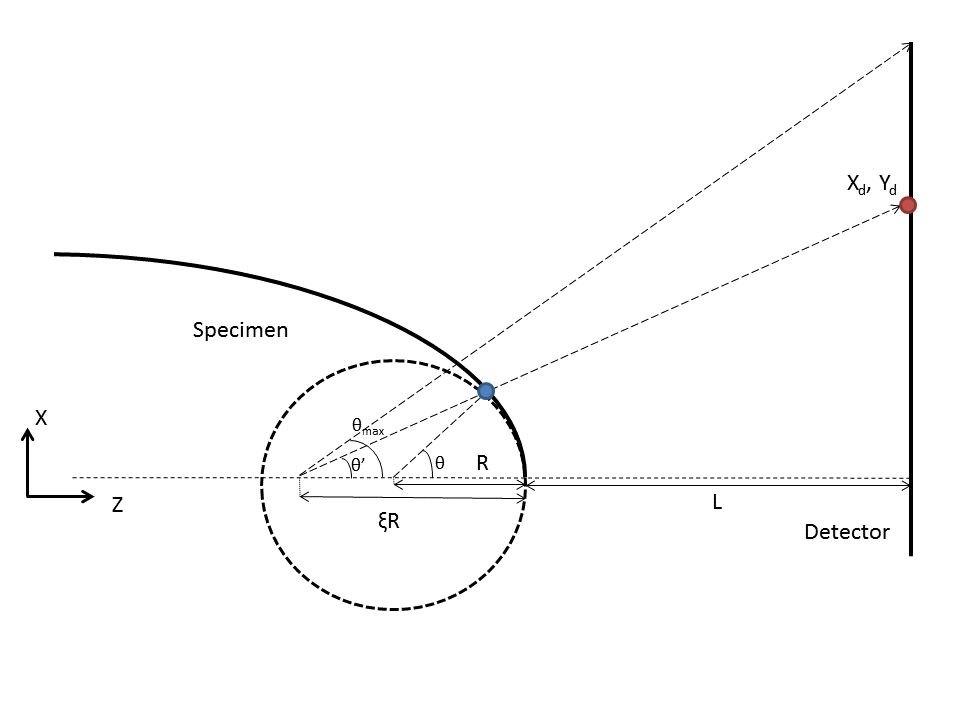
\includegraphics[width=\textwidth]{p3_projection}
	}
	\caption{Схематическое изображение точки-проекции: точка (X, Y) на наконечнике дает удар ($X_d$, $Y_d$). Определения углов в модели стереографической проекции.}
	\label{fig:p3_projection}
\end{figure} 
Координаты X и Y восстанавливаются с помощью стереографической проекции. Схема реконструкции представлена на Рисунке \cref{fig:p3_projection}. Прямая связь между двумя углами $\theta$ и $\theta$' и координатой Z может быть получена как:

\begin{equation}
	\label{eq:equation3_4}
	\theta = \theta' + \arcsin(\xi - 1)\sin{\theta'}
\end{equation}
\begin{equation}
	\label{eq:equation3_5}
	z_i = \frac{\Omega N_i}{Q R^2 \pi 2 {\sin^2(\theta_{max})}} + R (1- \cos{\theta})
\end{equation}

где $\theta$ - исходный угол запуска иона, который представляет собой реальный угол проекции, $\theta$' - угол, наблюдаемый после сжатия траекторий иона, Q - эффективность обнаружения, $N_i$ - номер обнаруженного атома. Угол $\theta_max$ - это максимальный угол обнаружения атомов. Уравнение \cref{eq:equation3_3} позволяет восстановить радиус в алгоритме Bas. Радиус впоследствии используется для восстановления координат. Важно отметить, что изменения kf играют важную роль в вычислении координаты Z, поскольку они влияют на значения обеих частей в сумме в \cref{eq:equation3_5}. Первая часть в \cref{eq:equation3_5} оказывает прямое влияние на координату Z. Второй (с ICF в $\theta$) - это поправка на кривизну поверхности. Следовательно, ICF влияет только на координаты X и Y. Чтобы продемонстрировать роль параметров реконструкции, одна и та же часть исследуемого образца была реконструирована с различными значениями $k_f$ и IFC (см. Рисунок \cref{fig:p3_3Dparts}). Как будет показано ниже, оптимальные значения $k_f$ и IFC могут быть выбраны, если реконструированная плотность материала образца приведена в соответствие с реальной.

\begin{figure}[htb]
	\centerfloat{
		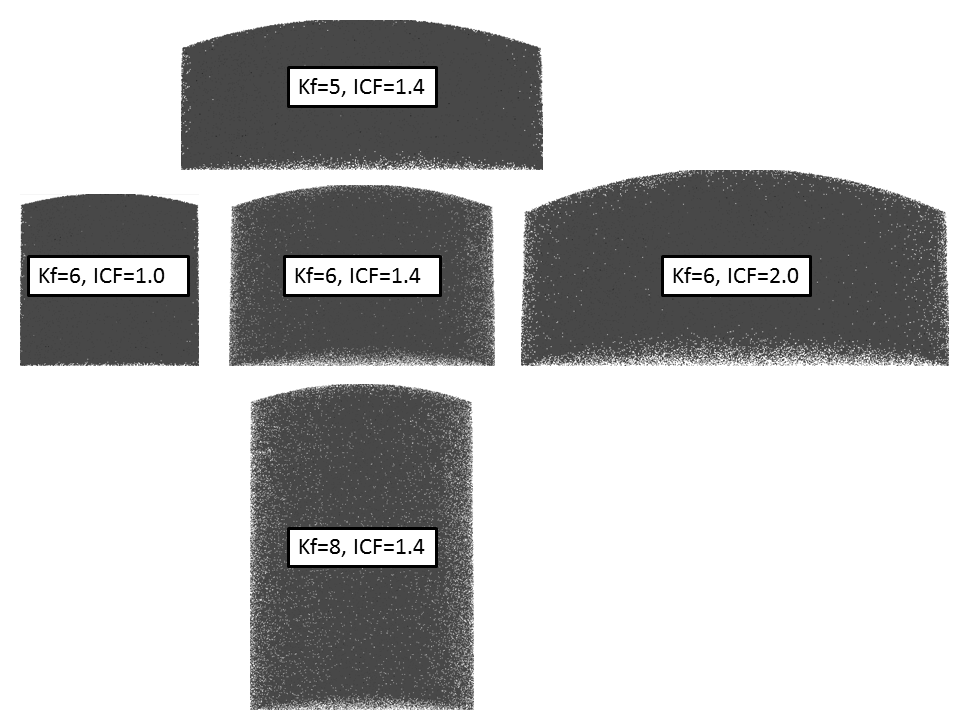
\includegraphics[width=\textwidth]{p3_3Dparts}
	}
	\caption{Карты атомов, построенные из одной и той же части исследуемого образца с различными параметрами $k_f$ и ICF}
	\label{fig:p3_3Dparts}
\end{figure}

\begin{figure}[htb]
	\begin{minipage}[b][][b]{0.49\textwidth}\centering
		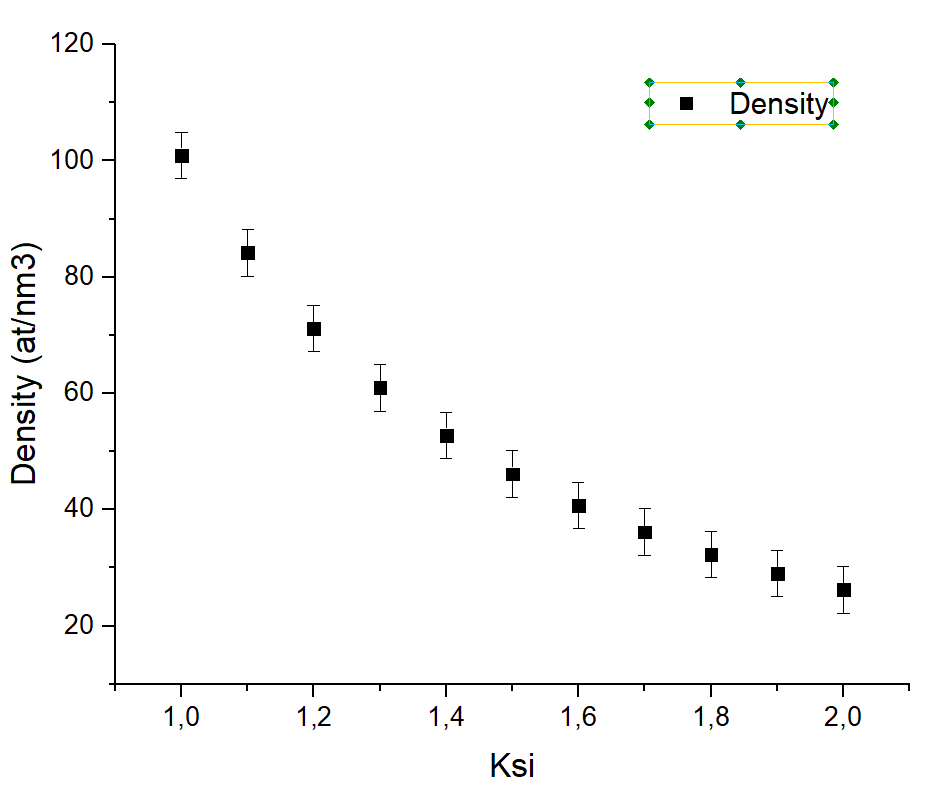
\includegraphics[width=\textwidth]{p3_ICFvsKsi} \\ а)
	\end{minipage}
	%\hfill
	\begin{minipage}[b][][b]{0.49\textwidth}\centering
		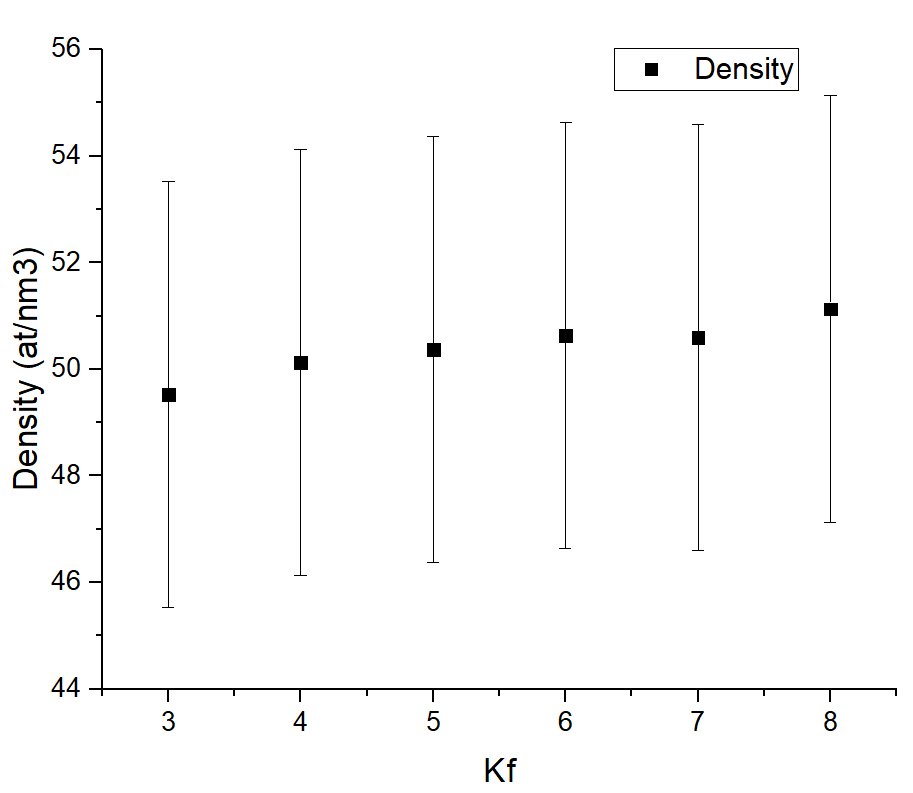
\includegraphics[width=\textwidth]{p3_ICFvskf} \\ б)
	\end{minipage}
	\caption{График атомной плотности как функции ICF (а). График атомной плотности как функции фактора поля $k_f$ (б)}
	\label{fig:p3_ICF}
\end{figure}

Следует отметить, что размер Z объема не изменяется при изменении ICF и фиксируется $k_f$, изменяются только радиус R и угол $\Theta$. Как объяснялось выше, это следствие выбранного алгоритма реконструкции. Как показано на Рисунке \cref{fig:p3_ICF} (б), атомная плотность не меняется с эволюцией $k_f$. Это связано с тем, что координаты X и Y пропорциональны радиусу, а Z обратно пропорциональна квадрату радиуса (см. Уравнения \cref{eq:equation3_1,eq:equation3_2,eq:equation3_5}). Таким образом, можно сделать вывод, что в алгоритме реконструкции $k_f$ и ICF можно откалибровать отдельно.
Принимая во внимание все перечисленные детали, предлагаем следующий алгоритм реконструкции. Первым шагом реконструкции является поиск динамического $k_f$. На значение $k_f$ напрямую влияет на все три координаты. Поэтому на данном этапе целесообразно использовать эмпирическую калибровку для восстановления кристаллических плоскостей. Второй шаг - это выбор динамического ICF, который практически не меняет расстояния в направлении Z. На этом этапе можно использовать плотность материала для определения правильной зависимости ICF. Мы предлагаем выбрать переменные параметры для согласования восстановленной плотности с реальной плотностью материала образца по всему объему.
Таким образом, при поиске ICF и $k_f$ используются известные значения, такие как межслоевые расстояния кристаллов и атомная плотность. Согласно работам групп Gault \cite{Gault11_Loi}, Loi \cite{Loi13} и Da Costa \cite{Hatzoglou19}, можно предположить, что зависимости ICF(U) и $k_f$(U), найденные для чистых материалов, будут одинаковыми по точности для сплавов.

Представленный АЗТ-анализ проводился на установке ПАЗЛ-3D в НИЦ Курчатовский институт - ИТЭФ \cite{scbibAPPLE}. В ПАЗЛ-3D используется лазерное полевое испарение, прямопролетная геометрия и программное обеспечение, разработанное в ИТЭФ. Образцы АЗТ получали электрохимическим методом с использованием стандартных электролитов. Форма кончика образцов контролировалась с помощью просвечивающего электронного микроскопа JEOL 1200 EX. В процессе сбора данных температура образца составляла 21 К, скорость сбора данных составляла от 2 до 6 атомов на 1000 лазерных импульсов, а энергия лазера составляла от 5 до 10 мВт с частотой 25 кГц. Для сплавов оптимальные условия испарения выбирались по методике, описанной в работе Разницына и др. \cite{scbibOptParamsYAFI}. Реконструкция данных проводилась с помощью программы КВАНТМ-3D \cite{KVANTM}. Для расчета масс-спектров с помощью этого программного обеспечения использовались процедуры автоматической калибровки и оптимизации \cite{Shutov19}.
Для восстановления массы и координат каждого атома использовалась программа КВАНТМ-3D. Для поиска зависимостей $k_f$(U) и ICF(U) были выбраны алюминий и вольфрам с гранецентрированной и объемноцентрированной кубической кристаллической структурой соответственно. Далее будут подробно описаны первый и второй этапы зависимостей поиска $k_f$(U) и ICF(U).

Как было написано выше, первым этапом алгоритма является поиск зависимости $k_f$ от напряжения на образце U. Объем образца разбивается на мелкие части по оси Z. Для каждой детали подбирается оптимальное расстояние между кристаллографическими плоскостями. Теоретические расстояния между атомными плоскостями соответствующих кристаллографических направлений взяты из приложения к книге Гаульта \cite{GaultBOOK}. Кристаллографические направления определялись по картам полевой десорбции. На Рисунке \cref{fig:p3_Alion} представлен пример карты полевой десорбции образца алюминия, полученной на АЗТ-детекторе.

\begin{figure}[htb]
	\centerfloat{
		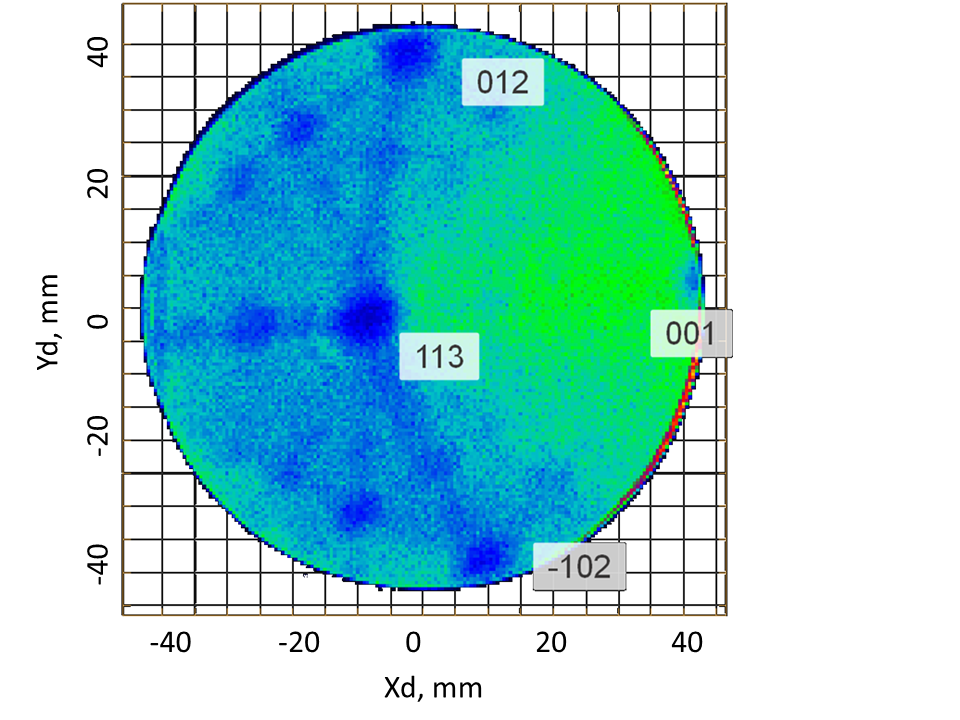
\includegraphics[width=\textwidth]{p3_Alion}
	}
	\caption{Карты полевой десорбции алюминиевого образца. Указаны кристаллографические направления}
	\label{fig:p3_Alion}
\end{figure} 

Для калибровки было выбрано ближайшее к центру детектора направление. Для большинства образцов этими направлениями были {111}, {001} и {113}. Информацию о межслоевых расстояниях, соответствующих выбранному направлению, можно взять из книги Гаульта \cite{GaultBOOK}. На Рисунке \cref{fig:p3_Alion} наиболее удобным направлением является {113} с расстоянием между атомными плоскостями около 1,2 \r{A}. Далее объем образца разбивался на мелкие части по оси Z. Каждая часть содержала 10-30 атомных плоскостей. Таким образом стало возможным найти значение $k_f$ для каждого небольшого кусочка образца. Напряжение на вершине в этих частях принималось постоянным для каждой из них. Полученные пары значений $k_f$ и напряжения U аппроксимировались функциональной зависимостью аналогичной в работе \cite{Hatzoglou19}. Пример аппроксимации данных выборки показан на Рисунке \cref{fig:p3_kf_vs_voltage}.

\begin{figure}[htb]
	\centerfloat{
		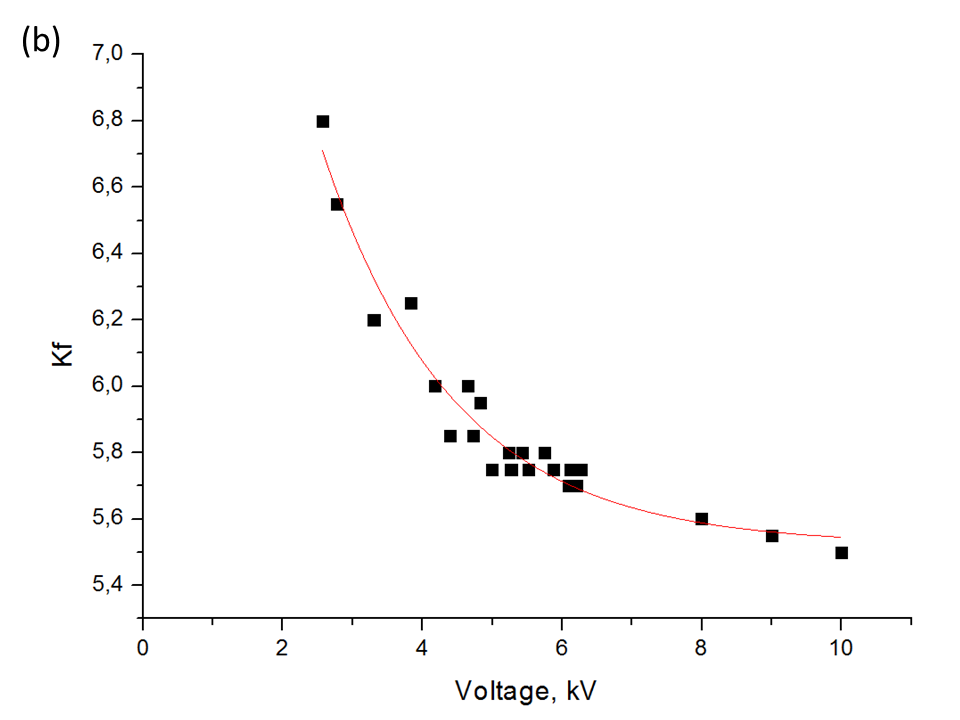
\includegraphics[width=\textwidth]{p3_kf_vs_voltage}
	}
	\caption{Экспериментальные данные $k_f$(черные точки) и наилучшая аппроксимирующая кривая (красная)}
	\label{fig:p3_kf_vs_voltage}
\end{figure} 

Описанная выше процедура была проведена для образцов из алюминия и вольфрама. $k_f$ как функция напряжения U была получена для каждой вершины. Из полученных данных была найдена общая зависимость $k_f$(U):

\begin{equation}
	\label{eq:equation3_6}
	k_f = (10 - C) + C\exp(- U * 5.3E-4)
\end{equation}

где C - константа подгонки. Значение постоянной зависит от состава материала. Например, для алюминия он равен 5,5, а для вольфрама - 4,5. Возможно, значение постоянной зависит от поля испарения материала. Явной разницы между коэффициентами в выражении \cref{eq:equation3_6} и углом стержня или начальным радиусом вершины не обнаружено. Полученная зависимость $k_f$(U) является экспоненциальной. Подобный характер зависимости был получен в работах Да Коста \cite{Hatzoglou19} и Лои \cite{Loi13}.
Следующим шагом после восстановления значения kf является корректировка значений ICF. Точность трехмерной реконструкции положения атомов в латеральном направлении недостаточна для идентификации кристаллической решетки. Согласно результатам, представленным на рис. 2, плотность может использоваться как критерий для получения значений ICF, обеспечивающих точность координат «сжатия» в плоскости XY. Тот же подход с разделением большого объема на мелкие части был использован для определения калибровочной кривой. Для каждой детали были найдены значение kf с использованием кристаллографических плоскостей и значение ICF с использованием плотности материала. Получена линейная зависимость ICF от напряжения на образце U. Зависимость ICF отличалась от полученных в аналогичных исследованиях \cite{Hatzoglou19, Gault11_Loi}. Это различие могло быть связано с режимом лазерного испарения в случае APPLE-3D в отличие от режима испарения с использованием локального электрода.
В программе анализа данных «КВАНТМ-3D» реализован инструмент «Линейная плотность» для построения графика атомной плотности вдоль выбранного направления. Атомная плотность рассчитывается вдоль выбранного направления. Для наглядности рисуется график с выбранным шагом. Примеры рассчитанных графиков плотности вдоль оси образца показаны на Рисунке \cref{fig:p3_Density_vs_depth} для алюминиевого образца с оптимизацией или без нее.

\begin{figure}[htb]
	\centerfloat{
		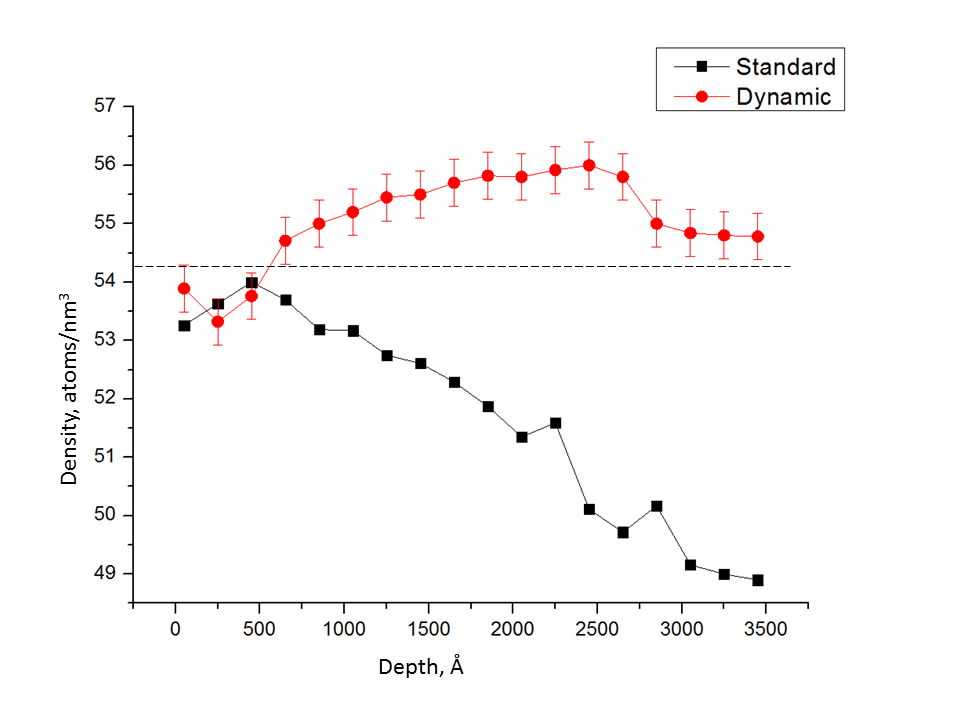
\includegraphics[width=\textwidth]{p3_Density_vs_depth}
	}
	\caption{Линейная атомная плотность вместе с образцом алюминия, полученная по стандартным протоколам и протоколам динамической реконструкции. Пунктирная линия показывает реальную плотность алюминия.}
	\label{fig:p3_Density_vs_depth}
\end{figure}

Необходимо скорректировать ожидаемую плотность для эффективности системы обнаружения для каждого прибора АЗТ, чтобы сравнить полученные значения с теоретическими. На использованной установке APPLE-3D установлена система детектирования с микроканальными пластинами с эффективностью детектирования ~ 90\%. В результате двух этапов калибровки были найдены динамические $k_f$ и ICF. Далее необходимо проверить эти зависимости на чистых материалах.

Предлагаемый протокол был протестирован на чистых материалах Al и W. Вольфрам имеет объемно-центрированную кубическую кристаллическую структуру с постоянной решетки около 3,16 \r{A} и 60,2 атома на кубический нанометр. Алюминий имеет гранецентрированную кубическую кристаллическую структуру с постоянной решетки около 4,05 \r{A} и 63,6 атома на кубический нанометр. Всего было исследовано 12 образцов алюминия и вольфрама. Для проверки точности реконструкции использовался специальный прибор для оценки расстояний между атомными плоскостями. Принцип этого инструмента основан на алгоритме распределения ближайших соседей k-го порядка \cite{GaultBOOK}. В программе КВАНТМ-3D этот инструмент называется «KNN-krist». Поиск соседей проводился только для атомов в выбранном направлении. Вместо дальнейшего поиска кластеров на гистограмму было нанесено распределение расстояний между ближайшими соседними атомами (см. Рисунок \cref{fig:p3_atomiccount_distance}). Расстояния между атомными плоскостями на разной глубине по оси Z были рассчитаны для всех образцов для стандартного и нового алгоритмов калибровки. Разница между этими алгоритмами показана на Рисунках \cref{fig:p3_PlanesDistance_depth,fig:p3_atomiccount_distance}.

\begin{figure}[htb]
	\centerfloat{
		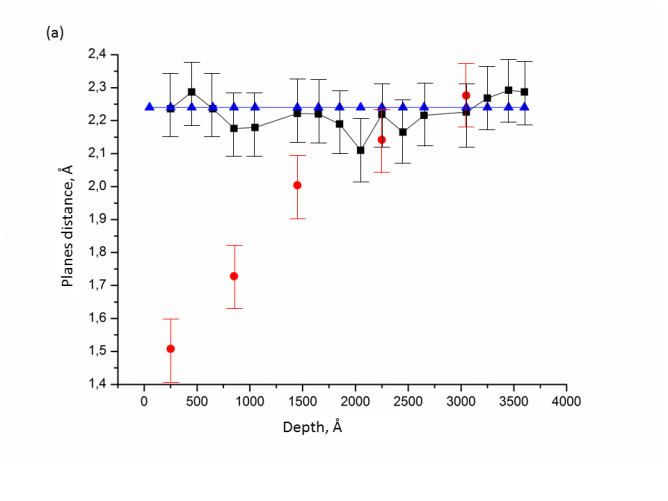
\includegraphics[width=\textwidth]{p3_PlanesDistance_depth}
	}
	\caption{Расстояние между атомными плоскостями как функция глубины по оси Z образца, полученное стандартным протоколом реконструкции (красный), динамическим протоколом $k_f$ и ICF (черный) и теоретическим значением (синий)}
	\label{fig:p3_PlanesDistance_depth}
\end{figure}
\begin{figure}[htb]
	\centerfloat{
		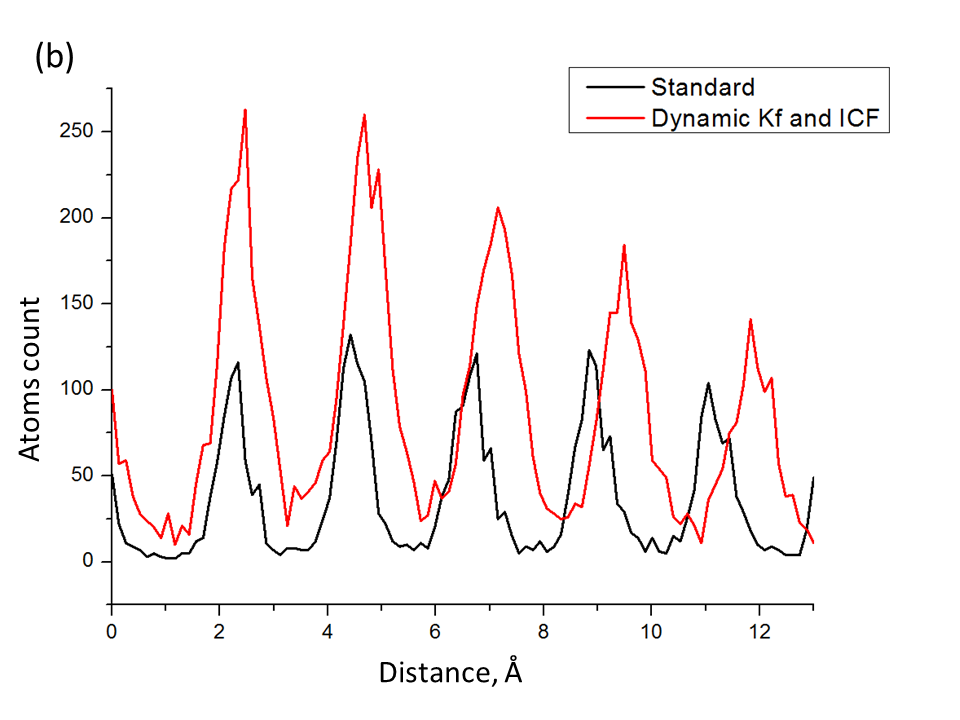
\includegraphics[width=\textwidth]{p3_atomiccount_distance}
	}
	\caption{Результат процедуры KNN-cryst для стандартных и динамических алгоритмов восстановления.}
	\label{fig:p3_atomiccount_distance}
\end{figure}

На Рисунке \cref{fig:p3_PlanesDistance_depth} видно, что ошибка в межплоскостных расстояниях, полученных в начале и в конце сбора данных АЗТ, может достигать 50\%. Важно отметить, что предлагаемые поправки могут значительно улучшить оценку размеров кластеров / фаз. Кроме того, учет этой поправки повлияет на точность расчета размеров переходных слоев, фаз и зерен. 
В этой статье был предложен алгоритм трехмерной реконструкции для данных АЗТ с использованием контроля плотности восстановленного материала. Этот протокол основан на алгоритме восстановления Баса. Отличительной особенностью этого протокола является проверка плотности материала вдоль выбранного направления для повышения точности восстановления данных. Динамические значения $k_f$ и ICF были измерены с использованием как кристаллографии, так и инструмента контроля плотности материала.

%\subsection{Подпараграф \cyrdash{} два}\label{subsec:ch3/sect33/sub2}

%Некоторый текст.














\clearpage
